 \hypertarget{index_intro_sec}{}\subsection{Introduction}\label{index_intro_sec}
This project is about using an W\+S2811 or W\+S2812 lightstribe with an A\+V\+R controller. It is possible to handle up to 250 L\+E\+Ds at the same time, so I chose an Atmega328p with enough R\+A\+M amount. If you want to handle less L\+E\+Ds you can use most parts of this project with every A\+V\+R. The A\+V\+R is programmed to receive the light data over U\+A\+R\+T so you can control the L\+E\+Ds by using a serial interface. The interface uses a specified simple protocol which is described in \hyperlink{index_protocol_sec}{Protocol overview} section. Everything has been developed in a university course to control the lights of a Christmas tree. In the original implementation there were some further components included. This is a simplified version of the implementation so that everyone can use it. As an example for controlling the L\+E\+Ds using a smart phone the \hyperlink{index_esp_sec}{control via E\+S\+P8266} section shows how this could be done by using a webserver on the E\+S\+P8266. You can use everything else that provide a serial interface (maybe connect with a bluetooth serial module). The structure of this documentation is split in a hardware part for the A\+V\+R that describes the basic hardware that should be used. The next part is about how the software is working on the A\+V\+R that handles the L\+E\+Ds and different effects. You may include some more stuff in your own. After that you can see a small protocol overview, where you find which command can be sent to the A\+V\+R to control the L\+E\+Ds. Be aware that at the initialization state all L\+E\+Ds are off. At the last point you can find an example how to use the implementation with an E\+S\+P8266 with a webserver. You will find the source code for the E\+S\+P8266 and the basic hardware setup.\hypertarget{index_usage_sec}{}\subsection{Basic usage}\label{index_usage_sec}
For using this implementation follow this steps\+: 
\begin{DoxyItemize}
\item set up the hardware as descriped in section \hyperlink{index_hardware_sec}{Hardware} 
\item set the \hyperlink{globals_8h_a43bafb28b29491ec7f871319b5a3b2f8}{F\+\_\+\+C\+P\+U} clock to the value for your hardware 
\item set the \hyperlink{ws2811lichterkette_8c_a62634036639f88eece6fbf226b45f84b}{B\+A\+U\+D} to the value you like, 76800 or 38400 are suggested 
\item compile your implementation (only O1 optimization is supported) 
\item program your A\+V\+R with your binaries 
\item set the clock divider fuse and the clock source fuse referring to your implementation 
\item send protocol data (see section \hyperlink{index_protocol_sec}{Protocol overview}) to the R\+X pin of the A\+V\+R over a serial device, e.\+g. an F\+T\+D\+I, E\+S\+P8266 or Arduino (U\+A\+R\+T is 8\+N1 on your chosen \hyperlink{ws2811lichterkette_8c_a62634036639f88eece6fbf226b45f84b}{B\+A\+U\+D}) 
\end{DoxyItemize}\hypertarget{index_hardware_sec}{}\subsection{Hardware}\label{index_hardware_sec}
The basic hardware you need is a A\+V\+R controller an some W\+S2811 or W\+S2812 L\+E\+Ds you want to control. The A\+V\+R controller should have an hardware U\+A\+R\+T, otherwise you need to write some code for a software serial. In the project we chose an Atmega328p that has enough R\+A\+M to control 250 L\+E\+Ds. The internal software structure buffers the color data for the L\+E\+Ds to achieve an accurate timing, see section \hyperlink{index_software_sec}{Software implementation}. The A\+V\+R can be used with the internal clock at 8 M\+Hz, remember to clear the clock divider fuse. Otherwise an external 8 M\+Hz or 16 M\+Hz clock source can be used, the definition \hyperlink{globals_8h_a43bafb28b29491ec7f871319b5a3b2f8}{F\+\_\+\+C\+P\+U} must be set to the frequency you chose (remember to set the fuses for an external clock source). As an example figure \hyperlink{index_one}{1} shows using an external 16 M\+Hz crystal. \label{index_one}%
\hypertarget{index_one}{}%
  
\begin{DoxyImage}
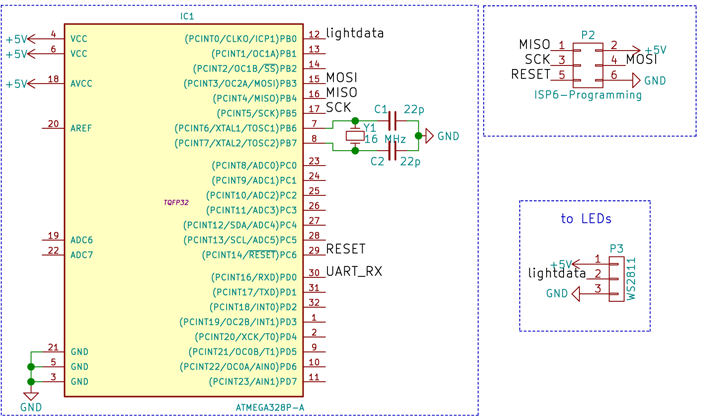
\includegraphics[width=\textwidth,height=\textheight/2,keepaspectratio=true]{Ws2811_Atmega328_schematic.png}
\caption{schematic of the A\+V\+R to controll W\+S2812/\+W\+S2811}
\end{DoxyImage}
  As you can see in the picture the A\+V\+R is programmed by using the I\+S\+P interface. The W\+S2812/\+W\+S2811 get the same voltage as the A\+V\+R, the light data is available at Pin\+B0, you may change this if you like. Referring to the L\+E\+Ds be aware of the current amount they may draw if every L\+E\+D has its full brightness. One W\+S2812 can draw up to 60 m\+A, so one meter with 30 L\+E\+Ds already need 1,8 A. If you want to control more L\+E\+Ds you may have a problem with the voltage drop along the stribe. For example if you control 180 L\+E\+Ds at six meters you not only need 10,8 A, furthermore you will probably have a voltage drop up to 2 V. To reduce the voltage drop you must increase the wire size with parallel wires to you stribe. You can see the voltage drop if you set all L\+E\+Ds to white. If you have only a small voltage drop every L\+E\+D will have the same color. If the voltage drop is too much you can see that the last L\+E\+Ds will have less blue color, so they will light in a warm white color even up to red. If you want to try out the L\+E\+Ds with the A\+V\+R you can build up everything on a breadboard. Pinheaders can be soldered easy at the light stribes as you can see in figure \hyperlink{index_two}{2}. \label{index_two}%
\hypertarget{index_two}{}%
  
\begin{DoxyImage}
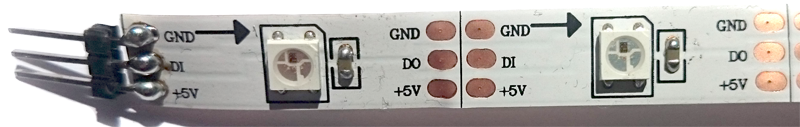
\includegraphics[width=\textwidth,height=\textheight/2,keepaspectratio=true]{WS2812.png}
\caption{W\+S2812 stribe with pin header}
\end{DoxyImage}
  The connect G\+N\+D to the common ground with the A\+V\+R, 5 V should be connected to a power supply that can handle the current you need. D\+I is the data in line, this should be connected to Pin\+B0 at the A\+V\+R. The stribe is like a big shifting register, all the data you sent is shifted bit by bit through the stribe. So D\+O is the data out pin, you see some data at this pin if all L\+E\+Ds before had already received their color data. The one wire protocol of the L\+E\+Ds is described in the next section \hyperlink{index_software_sec}{Software implementation}.\hypertarget{index_software_sec}{}\subsection{Software implementation}\label{index_software_sec}
If your hardware is ready you must flash your A\+V\+R device with the provided software. Therefore the I\+S\+P-\/6 connector should be used. To get the right timing remember to set the \hyperlink{globals_8h_a43bafb28b29491ec7f871319b5a3b2f8}{F\+\_\+\+C\+P\+U} definition to the frequency you are working at. Furthermore set the fuses of the A\+V\+R referring to your implementation. This means you have to clear the clock divider fuse and may have to change the clock source. I suggest to use the Atmel\+Studio to program your A\+V\+R and its fuses. ~\newline
 The W\+S2812/\+W\+S2811 are controlled by one data line that works with a one wire protocol. Because of the missing clock line the timing is really important, this can either be achieved by doing some trick with the hardware interfaces (e.\+g. using the spi interface) or by bit banging. In this implementation bit banging is used. To get a good timing all color data must be transmitted in one block that is not interrupted by some other code. The timing specifications of the W\+S2812/\+W\+S2811 L\+E\+Ds can be found in table \hyperlink{index_timingtable}{1} which refers to the datasheet.~\newline


\label{index_timingtable}%
\hypertarget{index_timingtable}{}%
 \begin{table}[h]\begin{TabularC}{3}
\hline
\rowcolor{lightgray}{\bf Information }&{\bf Timing }&{\bf Tolerance +/-\/ }\\\cline{1-3}
Transfer 1 Bit &High\+Time+\+Low\+Time=1,25 µs &600 ns \\\cline{1-3}
send 0, high time &0,35 µs &150 ns \\\cline{1-3}
send 0, low time &0,8 µs &150 ns \\\cline{1-3}
send 1, high time &0,7 µs &150 ns \\\cline{1-3}
send 1, low time &0,6 µs &150 ns \\\cline{1-3}
data transmission complete, low time &$>$50 µs &-\/ \\\cline{1-3}
\end{TabularC}
\centering
\caption{Timing table for W\+S2812/\+W\+S2811 one wire protocol}
\end{table}


The timing is done by setting the output and wait the required time by doing nothing (call assembly N\+O\+Ps). So it is important to compile the provided software at O1, other optimization levels may influence the timing. To send one bit (either high or low) two different macros are defined in \hyperlink{_lightstribe_8h}{Lightstribe.\+h} (S\+E\+T\+H\+I\+G\+H and S\+E\+T\+L\+O\+W), one L\+E\+D needs 24 color bits. The macros depend on the value of \hyperlink{globals_8h_a43bafb28b29491ec7f871319b5a3b2f8}{F\+\_\+\+C\+P\+U} you entered in \hyperlink{globals_8h}{globals.\+h}. Furthermore the header file Lightstrib.\+h declares a color struct to handle 24 bit colors (\hyperlink{structcolor24bit}{color24bit}) and three basic functions to control the L\+E\+Ds. The corresponding c file \hyperlink{_lightstribe_8c}{Lightstribe.\+c} implements these functions. The most important function is the \hyperlink{_lightstribe_8h_aac724dad670e4a26723daf71ce6a8d8a}{transmit2leds} function. This function and only this function transmits data to the stribe. All other functions either call this function or manipulate the color array. To achieve the right timing all effects and operations are done on a color array that stores the color information for the L\+E\+Ds. The information is sent to the L\+E\+Ds by calling transmit2leds with the lightdata pointer that points to an dynamically allocated array that stores the color information depending on the number of L\+E\+Ds you want to control. Therefore your color array must at least be able to contain 24 bits x your number of L\+E\+Ds. It can be bigger, what will allow you to create even more effects (e.\+g. if you rotate a rainbow array). So the effects that are implemented in \hyperlink{_led_effects_8c}{Led\+Effects.\+c} change the color array and afterwards the \hyperlink{_lightstribe_8h_aac724dad670e4a26723daf71ce6a8d8a}{transmit2leds} is called. The c file \hyperlink{_led_effects_8c}{Led\+Effects.\+c} not only contains effects but also different necessary functions for the effects and the serial color handling. The \hyperlink{_led_effects_8h_a55291315ab0f2ca8d508f0e9da1920a7}{colorconv8to24} function converts the received 8 bit colors from the serial port to 24 bit colors for the lightstribes. So you only sent 8 bit colors over the serial port to the A\+V\+R to reduce data size. Further information can be found in the \hyperlink{index_protocol_sec}{Protocol overview} section. The colors are decompressed with a simple \hyperlink{_led_effects_8h_ad67a4e660b5122ed454e101432bbdba0}{map} function you may know from Arduino. The main.\+c file initializes the hardware and handles the L\+E\+Ds. A serial interrupt stores the data temporary. If the data transmission is complete the main function will extract the information and set the new configuration for the lightstribe.~\newline
 The last points to be mentioned in this section are some things you need to be careful. The first thing is that the 8 bit colors are in an R\+G\+B 3-\/3-\/2 format. The 24 bit color format depend on the L\+E\+Ds. W\+S2812 L\+E\+Ds use a G\+R\+B color scheme while W\+S2811 use a R\+G\+B color scheme. This is important, to achieve the right color the protocol includes a bit that decides the color scheme. The right color is resolved by the decompressing function \hyperlink{_led_effects_8h_a55291315ab0f2ca8d508f0e9da1920a7}{colorconv8to24}. Another thing is that the colors are not linearized, what means that you cannot say that a color you got from a color table will be look like this. As an example you picked an orange from a 3-\/3-\/2 rgb color table. This orange will not be the same orange on the L\+E\+D stribe. This depends on many parameters so linearizing is too much effort and almost impossible (to achieve linearization you would have to measure each color, compare it and evaluate correction parameters).\hypertarget{index_protocol_sec}{}\subsection{Protocol overview}\label{index_protocol_sec}
This section gives an overview of the implemented serial protocol. The goal of the protocol was to be as simple as possible, to be easily implemented on the A\+V\+R and to use as less resources as possible. The figure \hyperlink{index_three}{three} shows the base structure of the protocol. \label{index_three}%
\hypertarget{index_three}{}%
  
\begin{DoxyImage}
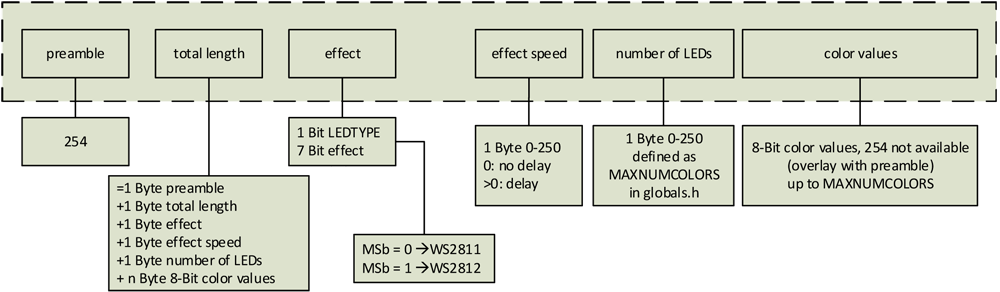
\includegraphics[width=\textwidth,height=\textheight/2,keepaspectratio=true]{Protoll_V1_2_engl.png}
\caption{W\+S2812 stribe with pin header}
\end{DoxyImage}
 \hypertarget{index_owneffects_sec}{}\subsection{Implement further effects}\label{index_owneffects_sec}
\hypertarget{index_esp_sec}{}\subsection{control via E\+S\+P8266}\label{index_esp_sec}
author\+: Florian Wank, 2016 